\subsection*{ISO-Kriterium Erlernbarkeit}
\begin{figure}[H]
    \centering
    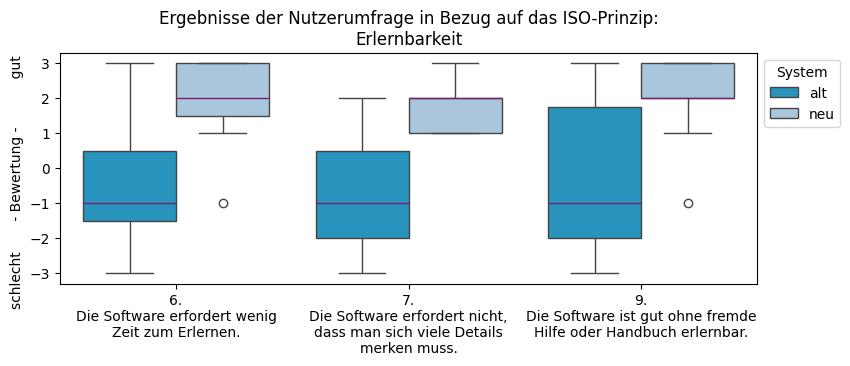
\includegraphics[width=1\linewidth]{Diagramme/pruemper_if.png}
    \caption{Auswertung der Fragen bzgl. Gestaltungskriterium Erlernbarkeit nach ISO 9241-110 (Ausschnitt aus \autoref{fig:pruemper_all})}
    \label{fig:pruemper_Erlernbarkeit}
\end{figure}

\noindent
t-Test von Fragen 6, 7 \& 9 sind signifikant (<0.5) - s. \autoref{tab:Nutzerbefragung:Differenz+ttest}\\
Boxplot: \autoref{fig:pruemper_Erlernbarkeit}